\chapter{\Large Iteración III: “Priorización de alertas”}
    En Security Onion y otros sistemas, el elemento descriptor que identifica y procesa a cada definición de incidente en particular es la regla. Las reglas comprenden una serie de campos que describen con precisión la naturaleza de un incidente dado y por lo tanto, existen tantas reglas como amenazas en circulación. \par
    Cuando un nuevo malware es descubierto por el equipo de algún CSIRT con la capacidad de investigación suficiente o reportado a un laboratorio apropiado para este fin, es posible realizar un estudio de sus características y una vez identificadas estas últimas, proceder a crear una regla y agregarla al repositorio correspondiente para que otros CSIRT actualicen sus IDS con esta nueva definición y así contar con un filtro (la regla) que permita detectar este malware. Las reglas tienen un conjunto de campos donde se detallan características del paquete y su contexto, tales como el puerto de origen y destino, protocolo empleado, dirección IP, etc y unos campos dedicados a la naturaleza del incidente (clasificación, mensaje, prioridad, etc). Algunos de estos campos son comunes a todas las reglas y permiten agruparlas para administrar eficientemente las alertas generadas cuando una regla coincide con la descripción de un incidente. Dado que estos campos también se pueden considerar observables, es posible utilizarlos por TheHive para gestionar incidentes y crear casos. \par

    \begin{section}{Verificación del requerimiento funcional 5: Definición de criterio para priorizar alertas.}
    Como se indicó anteriormente, la estructura de las reglas consisten en dos partes bien definidas: un encabezado (header) que es obligatorio  y un conjunto de campos opcionales. Dentro del header encontramos la acción (alerta, notificación, etc), el protocolo (tcp, udp), puertos de origen y destino, el sentido del evento (entrante o bidireccional) y las direcciones IP de origen y destino. \par
    La segunda parte de las reglas incluye dos tipos de campos: los que describen la naturaleza del evento y aquellos que contienen información del paquete de datos. Dentro del primer grupo encontramos aquellos tales como msg (descripción del evento), sid (id de la firma), classtype (clasificación de reglas o alertas), priority (prioridad de la firma y/o alerta), target (especifica de qué lado está el objetivo, es decir puerto de origen y puerto de destino), entre otros. El segundo grupo contiene datos extraídos que provienen desde de la capa de red hasta la de aplicación de la pila OSI. Se pueden mencionar a los campos “GeoIP” (localización geográfica de la IP), “Fragbits” (presencia del bit de fragmentación), “ACK” (presencia del campo ACK en paquete TCP), “itype” (número del tipo de mensaje ICMP), “http.method” (tipo de método HTTP usado), entre otros.
    \begin{figure}[H]
        \centering
        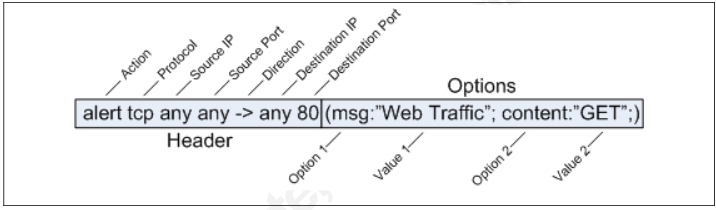
\includegraphics[width=0.7\textwidth]{./iteracion_3_imagenes/figura_41_estructura_regla.png}
        \caption{Estructura general de una regla}
        \label{fig:figura_41_estruc_regla}
    \end{figure}
    
    Como los campos están presentes en todas las reglas, es posible hacer uso de algunos de ellos para agrupar reglas que describen amenazas pertenecientes a un mismo grupo o categoría de malware, intentos de intrusión, reconocimiento, escalado de privilegios, etc y por lo tanto son útiles para gestionar los incidentes. \par
	Es posible configurar esta gestión a través de un archivo que relaciona campos como categorías de eventos con prioridades de la alerta generada. Este archivo llamado “classification.config” se encuentra bajo el directorio que almacena las reglas descargadas desde diversas fuentes; en particular relaciona los campos “classtype” con “priority”, de manera tal que cualquier regla cuyo campo classtype contenga a los descritos en este archivo, generará una alerta con prioridad definida también en este. De esta manera, es posible administrar un enorme número de reglas agrupadas en un reducido grupo de categorías y modificar el nivel de prioridad que tendrá en el sistema las alertas que generan. \par
	El objetivo de asignar distintos niveles de prioridad a las alertas generadas por los eventos que sucedan radica en la naturaleza de los eventos, su importancia y la gestión de la atención de los analistas del CSIRT. Esto se debe a las necesidades de optimizar el uso de los recursos técnicos y humanos del centro de respuesta a incidentes para cumplir de la manera más eficiente posible con los objetivos y políticas de la organización a la cual pertenece. De esta manera, la naturaleza de los incidentes determina su elegibilidad para una respuesta automatizada al tener en cuenta por un lado su estructura bien conocida y por el otro su alta tasa de repetición en un periodo determinado. En estos casos, sería inutil destinar valiosos recursos como la atención de un analista ya que conoce perfectamente la estructura del incidente y por lo tanto la respuesta apropiada o en aquellos casos en los que aún conocida su estructura, el incidente proviene en simultáneo de múltiples fuentes en muy poco tiempo, de manera que la capacidad humana de responder de a uno a la vez estaría tan sobrepasada que no sería efectiva. Estos son los casos de ataques de reconocimiento y los de denegación distribuida de servicio, entre otros. \par
	De aproximadamente cuarenta y siete (47) categorías de incidentes disponibles por defecto, consideramos para el máximo nivel de prioridad a siete clasificaciones dado su nivel de ocurrencia y nivel de impacto para la organización. 
    \begin{itemize}
        \item Web-application-attack: esta categoría engloba a un conjunto enorme de malware y ataques a nivel de capa de aplicación. Gusanos, ransomware, ataques de reconocimiento entre otras amenazas comparten esta categoría. Sobre el caso particular de los ataques de reconocimiento, se aplicaron filtros para separarlos de los demás ya mencionados. 
        \item Unsuccessful User: intentos repetidos de ganar acceso en ciertos activos e infraestructura de la organización.
        \item Attempted-dos: intentos de ataque de denegación de servicio y su variante distribuida
        \item Known client side exploit attempt: intento de ejecución de exploits en el lado del cliente.
        \item Exploit Kit Activity Detected: detección de actividad de un kit de exploits
        \item A suspicious filename was detected: detección de nombres de archivos sospechosos
        \item Network Trojan: detección de un virus troyano de red.
    \end{itemize}
    
    Para verificar el cumplimiento del requerimiento funcional 5, se procedió a editar el archivo  classification.config que se encuentra en el path /etc/nsm/rules/. En la Figura \ref{fig:squert-L2} se observa la detección de un incidente de reconocimiento en Squert. Este incidente pertenece a la categoría “attempted-recon” y en el archivo classification.config esta categoría tiene un nivel de prioridad 2, tal como se muestra en la figura (barra vertical naranja). Esto se puede observar con más detalle al analizar los campos de la alerta en Kibana, como se muestra en la Figura \ref{fig:Kibana-L2}. Se remarcó el campo “priority”, donde se vio que efectivamente el valor de la prioridad es 2.
    \begin{figure}[H]
        \centering
        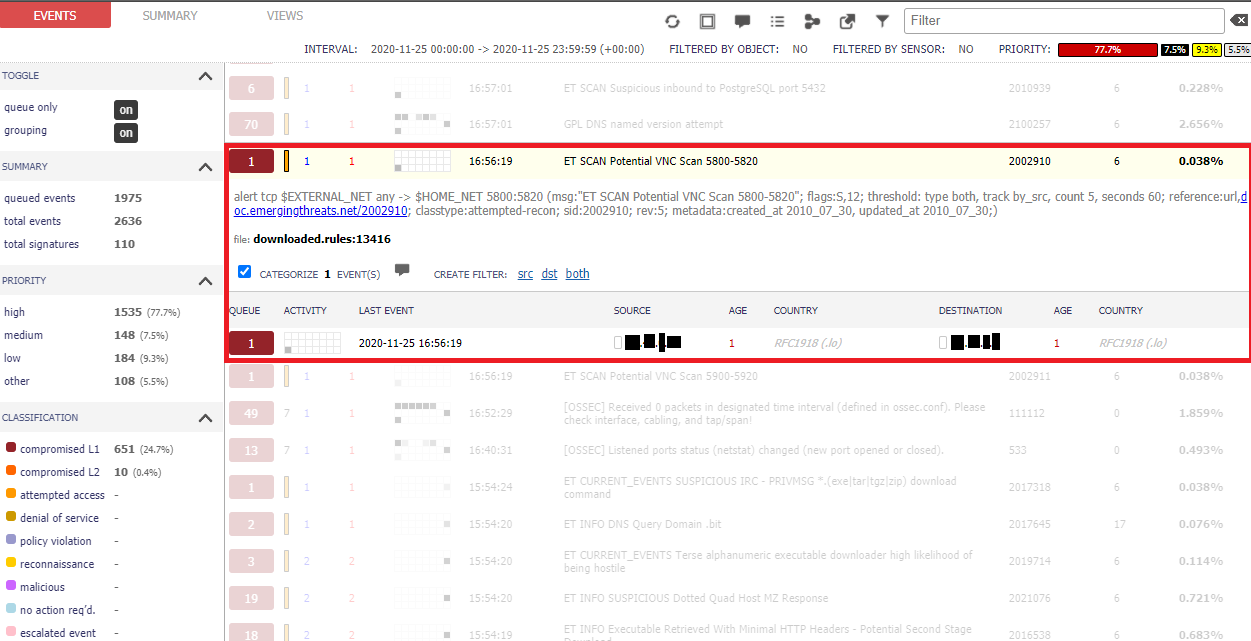
\includegraphics[width=1\textwidth]{./iteracion_3_imagenes/squert_ataque_vnc_L2-EDITADO.png}
        \caption{Incidente de reconocimiento en Squert. Prioridad nivel 2}
        \label{fig:squert-L2}
    \end{figure}
    \begin{figure}[H]
        \centering
        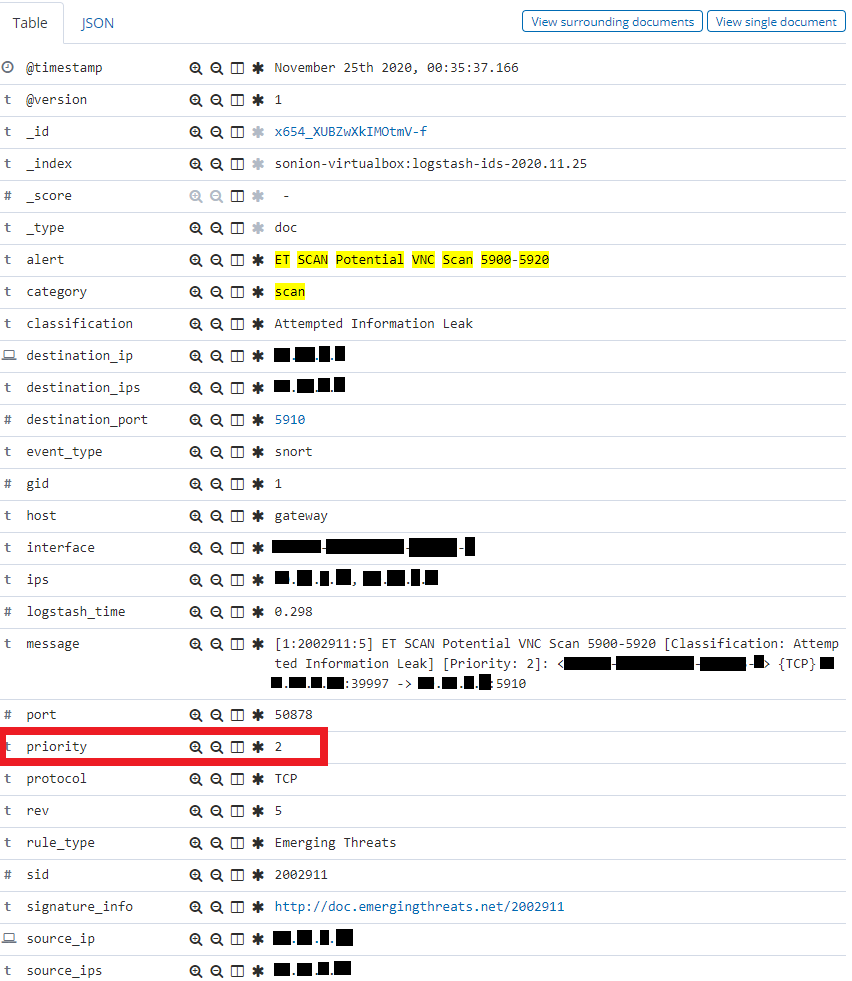
\includegraphics[width=1\textwidth]{./iteracion_3_imagenes/kibana_ataques_L2_1EDITADO.png}
        \caption{Incidente de reconocimiento en Kibana. Prioridad nivel 2}
        \label{fig:Kibana-L2}
    \end{figure}
    \FloatBarrier
    Se modificó el archivo \textbf{classification.config} para elevar el nivel de prioridad de los eventos asociados a la categoría “\textit{attempted-recon}”, que pasó del nivel 2 al nivel 1. Posteriormente se reiniciaron los sensores mediante el comando “\textit{so-sensor-restart}” y se procedió a comprobar los resultados de la modificación. Se repitió el ataque de reconocimiento y se pudo observar en las Figuras \ref{fig:squert-L1} y \ref{fig:kibana-L1} que Squert detectaba el ataque con prioridad 1 (barra vertical roja) y en Kibana se observó que el campo “priority” contenía el valor 1. Con esto se da por cumplido el requerimiento funcional 5.
    
    \begin{figure}[H]
        \centering
        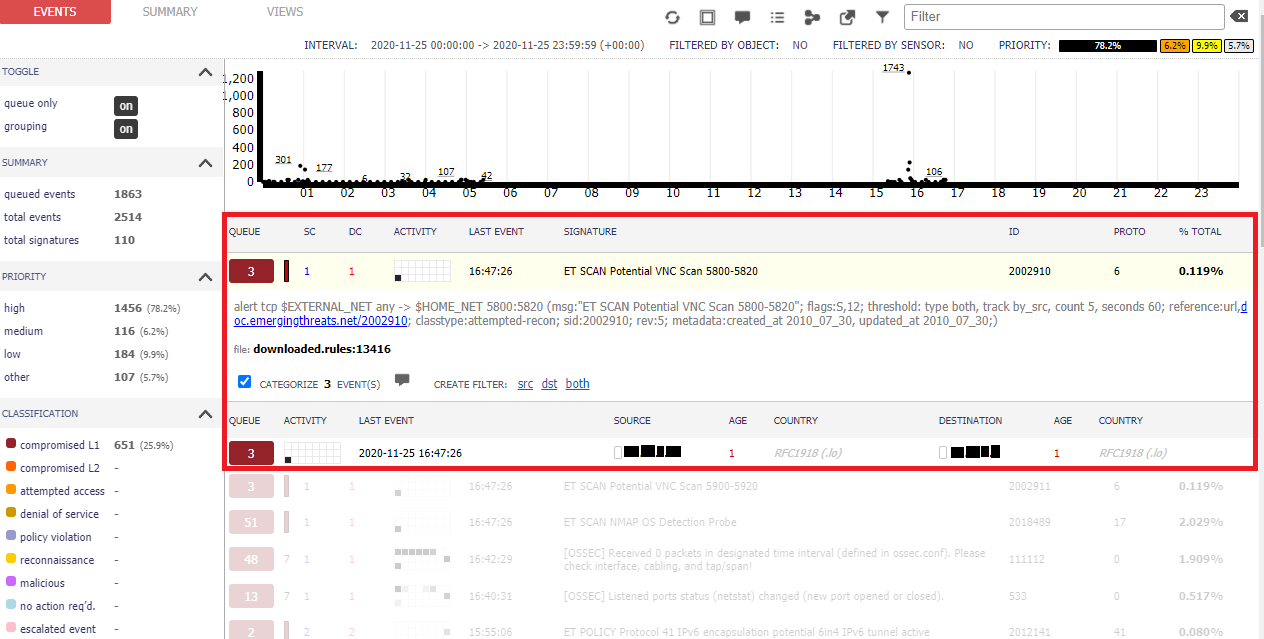
\includegraphics[width=1\textwidth]{./iteracion_3_imagenes/squert_ataque_vnc_L1-EDITADO.png}
        \caption{Incidente de reconocimiento en Squert. Nivel 1}
        \label{fig:squert-L1}
    \end{figure}
    \begin{figure}[H]
        \centering
        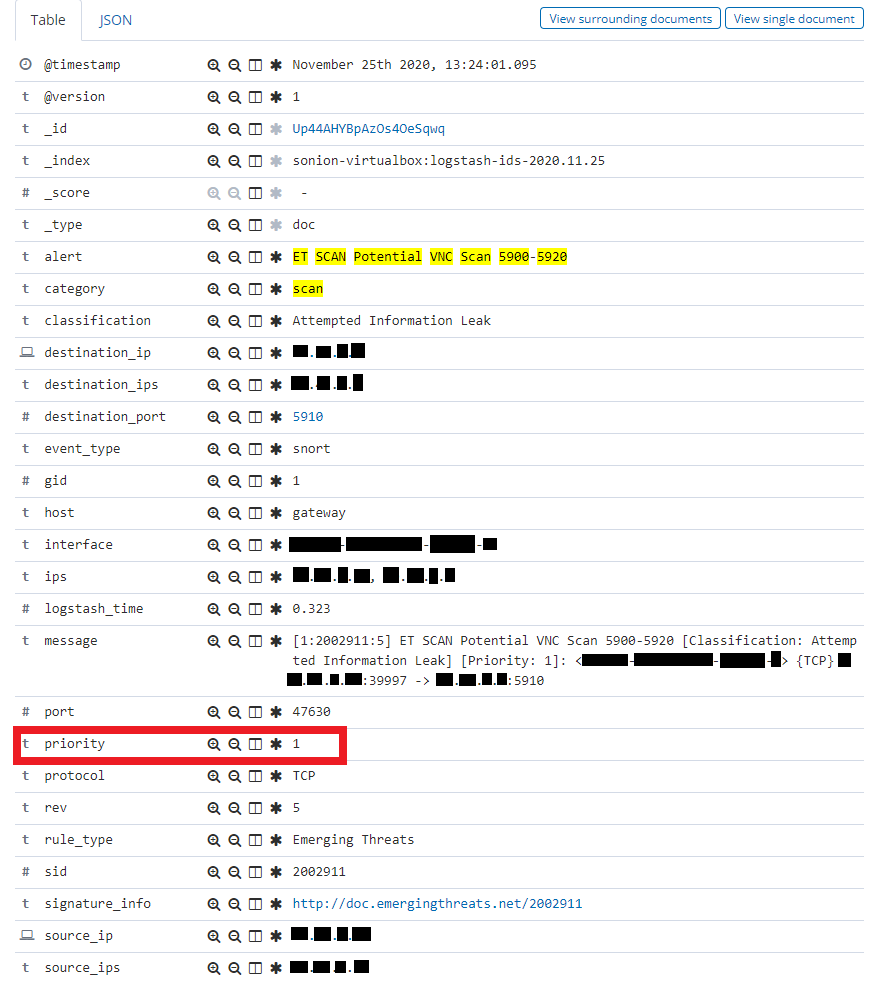
\includegraphics[width=1\textwidth]{./iteracion_3_imagenes/kibana_ataques_L2_2-EDITADO.png}
        \caption{Incidente de reconocimiento en Kibana. Nivel 1}
        \label{fig:kibana-L1}
    \end{figure}
    
    \end{section}
    
    \pagebreak
    \begin{section}{Requerimiento no funcional 4: Se requiere un despliegue automatizado de la solución}
    Para el despliegue automatizado de la solución se utilizó Ansible  2.8.4. Ansible es una herramienta de automatización de administración de servidores, utilizada en la organización donde se desplegó este proyecto. Esta herramienta permite ahorrar tiempo y esfuerzo al automatizar tareas repetitivas, disminuir errores y aumentar la productividad general cuando se trata del despliegue e instalación de infraestructura básica, como instalar sistemas operativos, realizar la configuración inicial de estos, etc. Es por esta razón que la organización requirió el desarrollo de scripts de instalación de nuestra solución en Ansible.\par
    En primer lugar, se desplegó una máquina virtual para probar el resultado de estos scripts. En esta máquina se instaló el sistema operativo Ubuntu Server 16.04 junto a los prerrequisitos para desplegar Ansible: Python en sus versiones 2.7 y 3.5, junto a su módulo pexpect (versión 4.7) y se configuraron las credenciales SSH entre esta máquina y el servidor desde el cual ordenamos el despliegue.\par
    Posteriormente se desarrolló un archivo de configuración de Security Onion para su despliegue. Si bien este archivo incluyó numerosos campos y variables, resaltan los correspondientes a la configuración de red, el tipo de rol (Master o Forward) y en base a esto las interfaces de monitoreo o administración, así como configuraciones de almacenamiento de logs, etc.\par
    Establecida la comunicación entre la máquina de destino y el servidor, se dio paso al inicio de la ejecución del script de Ansible. Para esto se ejecutó el comando “\textit{ansible-playbook -i hosts -l master so\_setup.yml --extra-var "target=sonionmaster"\hspace{1 mm} --ask-become-pass}”. En este caso, el comando especifica el despliegue de un nodo Master, sus flags y variables son las siguientes:
    \begin{itemize}
        \item \textit{ansible-playbook}: almacenan y ejecutan funciones de configuración, despliegue y orquestación de Ansible. Configura los pasos generales de un proceso de infraestructura IT y específica políticas para los sistemas remotos. 
        \item \textit{- i hosts}: flag que describe el inventario donde se encuentran los hosts. Esta variable \textit{host} es un archivo que describe las direcciones IP de las maquinas disponibles.
        \item \textit{- l}: opción utilizada junto al flag “\textit{-i}”, selecciona un subconjunto de hosts del inventario.
        \item \textit{--extra-var}: flag que configura variables adicionales como clave/valor o YAML/JSON. En nuestro ejemplo selecciona la opción \textit{sonionmaster} indica que se instaló un nodo Master de Security Onion.
        \item --ask-become-pass: flag que solicitó una contraseña de privilegio de usuario cuando fue necesario.
    \end{itemize}
    En el caso de la instalación de un nodo Forward, hubo que cambiar las opciones del  comando que se mencionó anteriormente. El resultado fue: “\textit{ansible-playbook -i hosts -l forward\_nodes so\_setup.yml --extra-var "target=sonionforward"\hspace{1 mm} --ask-become-pass}”. \par
    En el caso de la instalación de TheHive y Cortex, el proceso es análogo al descrito en el párrafo anterior.\par
    El comando para TheHive quedó de la siguiente manera: "\textit{ansible-playbook -i hosts -l thehive setup.yml --extra-var "target=thehiveuser"\hspace{1 mm}  --ask-become-pass}", mientras que en el caso de la instalación de Cortex, el comando resultante se muestra a continuación:
    "\textit{ansible-playbook -i hosts -l cortex setup.yml --extra-var "target=thehiveuser"\hspace{1 mm} --ask-become-pass}".\par
    Entre las acciones que realizó Ansible durante la ejecución de los scripts, se destacaron las de descargar e instalar los paquetes de Security Onion, para luego configurar el sistema operativo utilizando el archivo de configuración mencionado anteriormente. En el caso de la instalación de un nodo Forward, durante la configuración del sistema se debió ingresar la clave ssh para conectarse con el nodo Master.\par
    Finalmente se dio por satisfecho este requerimiento no funcional al comprobar que el sistema funcionaba correctamente.\par

    

    \end{section}